\documentclass[11pt,a4paper]{book}
\usepackage{Appunti_universitari}

\begin{document}
\title{Interazione uomo macchina}
\author{Jacopo De Angelis}
\maketitle

\pagebreak
\tableofcontents
\pagebreak

\chapter{Modulo 1: Concetti di base}
\section{Cos'è l'interazione uomo macchina?}
\begin{center}
Definizione standard 

\textit{"HCI (Human-Computer Interaction) è una disciplina che si occupa della progettazione, realizzazione e valutazione di sistemi interattivi con capacità computazionali destinati all'uso umano e dello studio dei principali fenomeni che li circondano"} - \textit{Associacion for Computing Machinery}
\end{center}

L'usabilità di un sistema è spesso trascurata all'interno dell'ambito lavorativo italiano, non per faciloneria ma perchè le risorse da adibire a questo ambito sono una spesa che non viene vista come essenziale nella produzione del valore per andare avanti. 

Il problema viene aggravato dall'outsourcing verso paesi dove il costo del lavoro sia inferiore e, ultimamente, anche da sistemi di ML che sono in grado, con grado di precisione sempre maggiore grazie al deep learning, di sviluppare codice funzionante. Ma cosa viene assegnato ai lavoratori esterni? Ciò che è altamente formalizzato, in modo da lasciare poche possibilità di variazione dalle richieste dei clienti.

Cosa rimane difficile da esternalizzare? Il contatto del cliente, sia durante la prima raccolta di requisiti funzionali, sia le successive interazioni con esso per cambiamenti incrementativi, variazioni di funzionalità o feedback.

L'usabilità è quella caratteristica che rende "facile la vita" al cliente.

\noindent\rule{\textwidth}{1pt}
\begin{center}
\textit{Piccola digressione}
\end{center}
\textbf{Perchè la concorrenza moderna rende sempre più importante l'analisi dell'interazione uomo macchina?}

In un contesto monopolistico le aziende non sono invogliate a produrre la soluzione "migliore"\footnote{Dove per migliore si intende quella che prende in considerazione più metriche come usabilità, efficienza, efficacia, design, ecc} ma solo quella più efficiente a livello di costo marginale.   

Cosa vuole dire questo? Che nella moderna concorrenza derivante da sistemi di sviluppo sempre più semplici e un'offerta più rapida tramite internet, per ottenere quote di mercato le aziende devono iniziare a pensare non solo al "funziona?" ma anche al "come lo faccio funzionare?"
\\\noindent\rule{\textwidth}{1pt}

\textbf{"Qui non si impara a fare delle interfacce usabili, si impara a riconoscere l'usabilità delle interfacce"} ovvero impariamo strumenti che ci possono portare a fare delle belle interfacce, certo, ma soprattutto ci permette di riconoscere cosa renda \underline{buona} un'interfaccia.

La disciplina nasce negli anni '80 ma l'interazione con le macchine (intese come calcolatori) esiste dagli anni'40, semplicemente prima l'utente era ultra specializzato mentre ora quasi tutti possono accedere ad un PC e con questo interagire tramite un'interfaccia.

Dal 1983 si tiene la conferenza annuale \href{https://dl.acm.org/conference/chi}{ACM CHI}. In questi casi tre aree disciplinari si incontrano:
\begin{itemize}
	\item ergonomia
	\item informatica
	\item psicologia comportamentista
\end{itemize}
\begin{figure}[h!]
	\begin{center}
		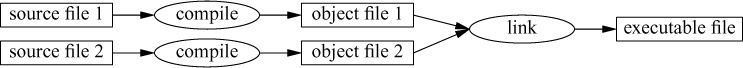
\includegraphics[scale=0.6]{img/001.jpg}
		\caption{HCI e le sue componenti}
		\label{fig: 001}
	\end{center}
\end{figure}
Dobbiamo ricordare sempre una cosa: dobbiamo lasciarci alle spalle l'utente ideale, l'utente senza faccia e senza capacità, e iniziare a pensare all'utente reale, ovvero a chi, idealmente, è diretta la nostra interfaccia. \underline{L'utente non siamo noi}. Proprio per questo le interviste, i test con esterni, i mockup sono utili, perchè ci permettono di vedere la nostra idea attraverso gli occhi di altri. Esempio banale: la nostra interfaccia basata sul colore potrebbe essere altamente confusionaria per un daltonico. Un'applicazione mobile dove tutti i comandi sono sulla destra potrebbe essere difficile da usare per un mancino.

\textbf{Ergonomia cognitiva}: studio dell'interazione tra l'uomo e gli strumenti per l'elaborazione di informazioni studiando i processi cognitivi coinvolti (percezione, attenzione, memoria, pensiero, linguaggio, emozioni) e suggerendo delle soluzioni per migliorare tali strumenti.

\section{Perchè è difficile progettare perchè l'interazione sia "buona"?}
Ci sono tre ragioni, idealmente:
\begin{enumerate}
	\item \textbf{La varietà dei sistemi interattivi}: cellulari, computer, cloche, macchine da cucina, tablet...
	\item \textbf{La varietà degli utenti}: fasce d'età, background culturale, condizioni mediche...
	\item \textbf{La varietà degli scopi e degli usi}: contesti formativi, ludici, lavorativi e usi tramite dispositivi diversi, in luoghi differenti...
\end{enumerate}

\begin{center}
\textbf{\textit{Noi studieremo come progettare per la varietà e al volto delle procedure.}}
\end{center}

\section{Temi dell'HCI}
\begin{itemize}
	\item Criteri, metodi e strumenti per la \textbf{progettazione dell'interazione} fra esseri umani e sistemi interattivi. L'interazione è il contesto nel quale interagiamo;
	\item Criteri, metodi e strumenti per la \textbf{valutazione dell'usabilità} dei sistemi interattivi;
	\item Progettazione di nuove \underline{tecniche di interazione} (dall'hololens ai sistemi che sfruttano i sistemi nervosi);
	\item Valutazione dell'\textbf{impatto dell'automazione} nei contesti umani
	\item \textbf{Sistema socio-tecnico}
\end{itemize}
Per valutazione dell'\textbf{impatto} ci si riferisce a due tipi di impatto:
\begin{itemize}
	\item a breve termine: sui singoli e nel qui ed ora (usabilità)
	\item a medio-lungo termine: sono conseguenze inattese sulla collettività
\end{itemize}

\noindent\rule{\textwidth}{1pt}
\begin{center}
	\textbf{Errore comune}
\end{center}

L'usabilità è un tipo di effetto/impatto sugli utenti (sui singoli utenti), NON è una caratteristica intrinseca di un sistema). Per questo non si può valutare l'usabilità senza il coinvolgimento degli utenti (di vario tipo) e sarebbe meglio valutarla in un contesto più simile possibile a una situazione reale.

Ricordiamo che l'usabilità non è solo un concetto di "correttezza funzionale" ma anche di "facilità d'uso".

\noindent\rule{\textwidth}{1pt}

Non si può parlare di impatto se non si parla di su che sistema socio-tecnico dovrà avere un impatto.
\section{Sistema socio-tecnico}\label{par: sistema sociotecnico}
Banalmente possiamo dire che è un contesto di umani che lavorano assieme tramite delle tecnologie. Quindi:
\begin{itemize}
	\item è un sistema, "un insieme di elementi interrelati ed eventualmente mutuamente dipendenti che, agli occhi di un osservatore esterno, appaiono come un'entità unitaria ma collettiva, con caratteristiche e comportamento proprio, solitamente autonomo ed intenzionale (cioè volto ad un obiettivo)";
	\item Un sistema in cui la componente umana  (sociale) e quella tecnica (tecnologica) sono inestricabilmente legate tra loro e la loro interazione porta a fenomeni emergenti impredicibili. Attenzione che tecnica è un termine generico proprio per intendere tutti gli strumenti, che siano fisici o dell'ingegno. In più si parla di interdipendenza perchè lo strumento è fermo senza qualcuno che lo usa, l'umano è fermo se non ha uno strumento per agire;
	\item è un concetto di invarianza di scala, ovvero il concetto non cambia in base alla grandezza dell'ambiente sociale
\end{itemize}
Come progettisti dobbiamo essere pronti all'imprevisto, ovvero all'utente che usa lo strumento non nel modo prescritto.

STS\footnote{Socio-technical system} thinking: un approccio che è consapevole che le due componenti si integrano bene (fit) e si "ottimizzano" solo congiuntamente in configurazioni subottime (joint optimization). Bisogna quindi pensare al sistema nella sua interezza e come le parti si integreranno.

Non si deve pensare solo alla qualità degli strumenti ma anche al contesto nel quale vanno usati. Ad esempio la soddisfazione del lavoratore può migliorare l'interazione. Questo va a contribuire alla qualità della configurazione. 

L'introduzione di una tecnologia in un contesto (sociale) è parte di un processo di cambiamento operante su più piani. Seguendo ciò che è detto prima si capisce che bisogna pensare non solo alla nostra tecnologia a livello funzionale (sistema tecnico) quando pensiamo all'interazione ma anche a dove andrà inserita e come migliorare quel contesto (sistema sociale).
 
\subsection{Proprietà emergenti}
Sono di due tipi:
\begin{itemize}
	\item \textbf{Sono proprietà funzionali}, riguardano il funzionamento dell'intero sistema una volta che tutte le sue parti, assembrale come devono, funzionano bene.
	\item \textbf{Sono proprietà non funzionali} che riguardano quanto bene opera il sistema in un determinato ambiente/contesto. Un elenco non esaustivo è affidabilità, sicurezza, performance, sicurezza, usabilità, comfort. (E.g. le informazioni sono giuste ma non aggiornate in un sistema medico, perchè? Perchè non era comodo farlo, quindi veniva visto più come un obolo rispetto ad uno strumento utile, vuole dire che è progettato male a livello di usabilità)
\end{itemize}

\begin{center}
	\textit{L'emergenza è quando la somma delle parti vale più (a livello di usabilità) delle parti singole (e.g. una bici e le sue parti)}
\end{center}

\subsection{Conseguenza inattesa}
Iniziamo con un esempio, l'effetto Peltzman: l'introduzione obbligatoria del casco per i ciclisti rendeva questi più spericolati e anche i conducenti di macchina vedendone uno col casco. In più nei luoghi dove non c'era una distinzione netta tra marciapiede e carreggiata, gli automobilisti rallentavano automaticamente, riducendo il rischio di incidenti, questo perchè non potevano ideare una "zona sicura" da evitare ma per il resto vivere la strada come loro. Tutto ciò perchè gli umani tendono a bilanciare il rischio.

\noindent\rule{\textwidth}{1pt}
\begin{center}
	\textbf{Conseguenza inattesa}
\end{center}

Una conseguenza inattesa è quella cosa che può anche andare in maniera contro intuitiva rispetto alla progettazione, e.g. un social network fatto per conoscersi che diventa la base per le proteste di Washington.

\noindent\rule{\textwidth}{1pt}

Un tipo di conseguenza inattesa è il overreliance, ovvero il fatto di affidarsi maggiormente allo strumento a causa dei feedback positivi. Ci sono due tipi:
\begin{itemize}
	\item \textbf{Overdependence}: mancanza di autonomia, abuso e uso al di là dei bisogni effettivi, mancanza o ignoranza di un piano di contingenza, ovvero come eseguire un compito senza l'uso della tecnologia in esame.
	\item \textbf{Overconfidence}: pensare che non ci saranno mai problemi, non ci saranno mai danni derivanti dall'uso e non si potrà mai sbagliare.
\end{itemize}

La \textbf{complacency è la fiducia che il sistema tecnico funzionerà sempre come è stato progettato}, riducendo così l'attenzione durante l'utilizzo (e.g. le macchine a guida autonoma che richiedono l'attenzione del conducente ma questo le ignora perchè sicuro del funzionamento). è legata ai processi di monitoraggio.

L'\textbf{automation bias è l'eccessiva fiducia nella risposta} del supporto alle decisioni e quindi causa di errori di omissione o di azione quando i sistemi sono imperfetti (e.g. la calcolatrice che deve rispondere correttamente, non può essere altrimenti). è legato ai processi decisionali. \label{par: automation bias}

Le conseguenze inattese non sono intrinsecamente positive o negative, è solo la registrazione di un effetto non previsto.


Progettare sistemi usabili è progettare per l'uso, quindi per qualcosa che il progettista non controlla e che dipende dall'utente e da quello che fa. Per progettare sistemi usabili non esistono metodologie, è meglio:
\begin{itemize}
	\item imparare per imitazione e per esperienza, diventando così capaci di basarsi sulla seconda per allontanarsi dalla prima
	\item essere creativi ma non troppo per non disorientare l'utente che non avrebbe basi conoscitive
	\item valutare il proprio sistema coinvolgendo utenti veri
	\item essere progettisti responsabili, ovvero ragionare sulle conseguenze impreviste,Essere progettisti responsabili significa sapere che il proprio sistema sarà il componente di un sistema socio-tecnico che può stravolgere o comunnque modificare.
	\item aspettarsi che il lavoro possa avere conseguenze inattese e lavorare per minimizzarne l'impatto
\end{itemize}

\section{Usabilità}
\subsection{Bassa usabilità = danni e problemi}
Vari tipi di bassa usabilità:
\begin{itemize}
	\item gli utenti non capiscono come svolgere i propri compiti con il sistema
	\item il sistema presenta un'eccessiva quantità di funzionalità e opzioni (low use)
	\item gli utenti non capiscono cosa il sistema stia facendo (poca trasparenza)
\end{itemize}

\subsection{La colpa è dell'utente o del progettista?}
La prima idea è che se il progettista ha creato il sistema a prova di stupido, ci siano tutte le guardie, gli avvisi e le informazioni necessarie allora la colpa sia dell'utente se qualcosa va storto. Nella storia di Dedalo e Icaro viene automatico pensare che Dedalo (il progettista) ha ragione, ha detto tutto a suo figlio e l'altro comunque è andato contro di ciò.

Certo, la colpa è qualcosa che può essere arginato tramite i termini d'uso, "qualsiasi utilizzo fuori da queste linee guida non è nostro problema", per la legge saremmo a posto ma ciò non cambia un dettaglio: se l'utente ha sbagliato c'è la possibilità che siamo stati noi a progettare male l'esperienza. "Mica gli ho detto io di mettere le dita così vicino alla lama dell'affettatrice" ma hai pensato "se il salume diventasse troppo piccolo le dita si avvicinerebbero troppo alla lama, meglio inserire un sistema comodo per spostarlo"?

Gli oggetti ben progettati sono facili da interpretare e comprendere: contengono indizi visibili (affordances) del loro funzionamento. Vedremo successivamente cosa voglia dire. Un esempio è l'indicatore in tempo reale di robustezza della password.

\noindent\rule{\textwidth}{1pt}
\begin{center}
	\textbf{Affordance (invito all’uso)}
\end{center}

La relazione tra le azioni possibili di un agente in un determinato ambiente.

\noindent\rule{\textwidth}{1pt}

Gli oggetti progettati male possono essere difficili e frustranti da usare: non offrono indizi o ne danno di sbaglianti, oppure sono stati progettati curando l'estentica più che la funzionalità.

\subsection{Come capire a livello generico se l'interfaccia è chiara?}
Uno dei metodi più semplici è tracciare una linea tra le interazioni per vedere quanto rispetti un ordine di lettura. Possiamo anche basarci su quanti ostacoli alla comprensione ci siano, ad esempio pulsanti che non fanno capire cosa facciano, spiegazioni verbose e non basate su simboli, rendendo difficile l'interpretazione per una persona che non sa leggere la lingua. 

\subsection{Concetti estremi di (non) usabilità}
\subsubsection{Porta di Norman} \label{par: porta di norman}
\href{It's not you. Bad doors are everywhere.}{https://www.youtube.com/watch?v=yY96hTb8WgI}

Una porta di Norman è una porta il cui design suggerisce un'azione contraria a quella da fare o che richiede un segnale per spiegare come usarla.

Uno dei principi che possono andare in correzione qua è la "visibilità", ovvero la possibilità di scoprire quali azioni possano essere eseguite. Prendiamo un attimo come esempio i touchpad del computer: guardandoli non permettono di comprendere cosa un singolo, doppio o triplo tocco possano fare, non c'è quindi scopribilità.

L'altro è il "feedback", ovvero un segnale che permetta la comprensione di cosa sia successo.

"La porta ideale è quella per la quale non devo pensare come aprirla"


\noindent\rule{\textwidth}{1pt}
\begin{center}
	\textbf{Porta di Norman}
\end{center}

La tendenza del progettista a concepire oggetti o sistemi che non invitano all'uso (e all'uso corretto) sulla base di elementi visuali o indicazioni chiare (affordance), affidandosi quindi solo alla memoria, all'esperienza o all'intuizione e incontrando spesso il disorientamento o il fraintendimento dell'utente.

\begin{center}
	\textbf{Discoverability (visibilità)}
\end{center}

Permette all’utente di individuare facilmente qual è la funzione dell’oggetto, e quindi riconoscere se è adatto allo scopo prefissato. È il risultato dell’applicazione di tutti gli altri principi elencati.

\begin{center}
	\textbf{Feedback (reazione)}
\end{center}

É l’insieme di risposte che il sistema comunica all’utente, in base alle azioni effettuate fino a quel momento.

\noindent\rule{\textwidth}{1pt}

\subsubsection{Toilette di Floyd}\label{par: toilette di Floyd}
É la serie di istruzioni della toilette in Odissea nello Spazio.

Una toilette di floyd è un qualcosa di progettato in maniera così poco intuitiva per il quale devo fornire una serie di istruzioni.
\begin{figure}[h!]
	\begin{center}
		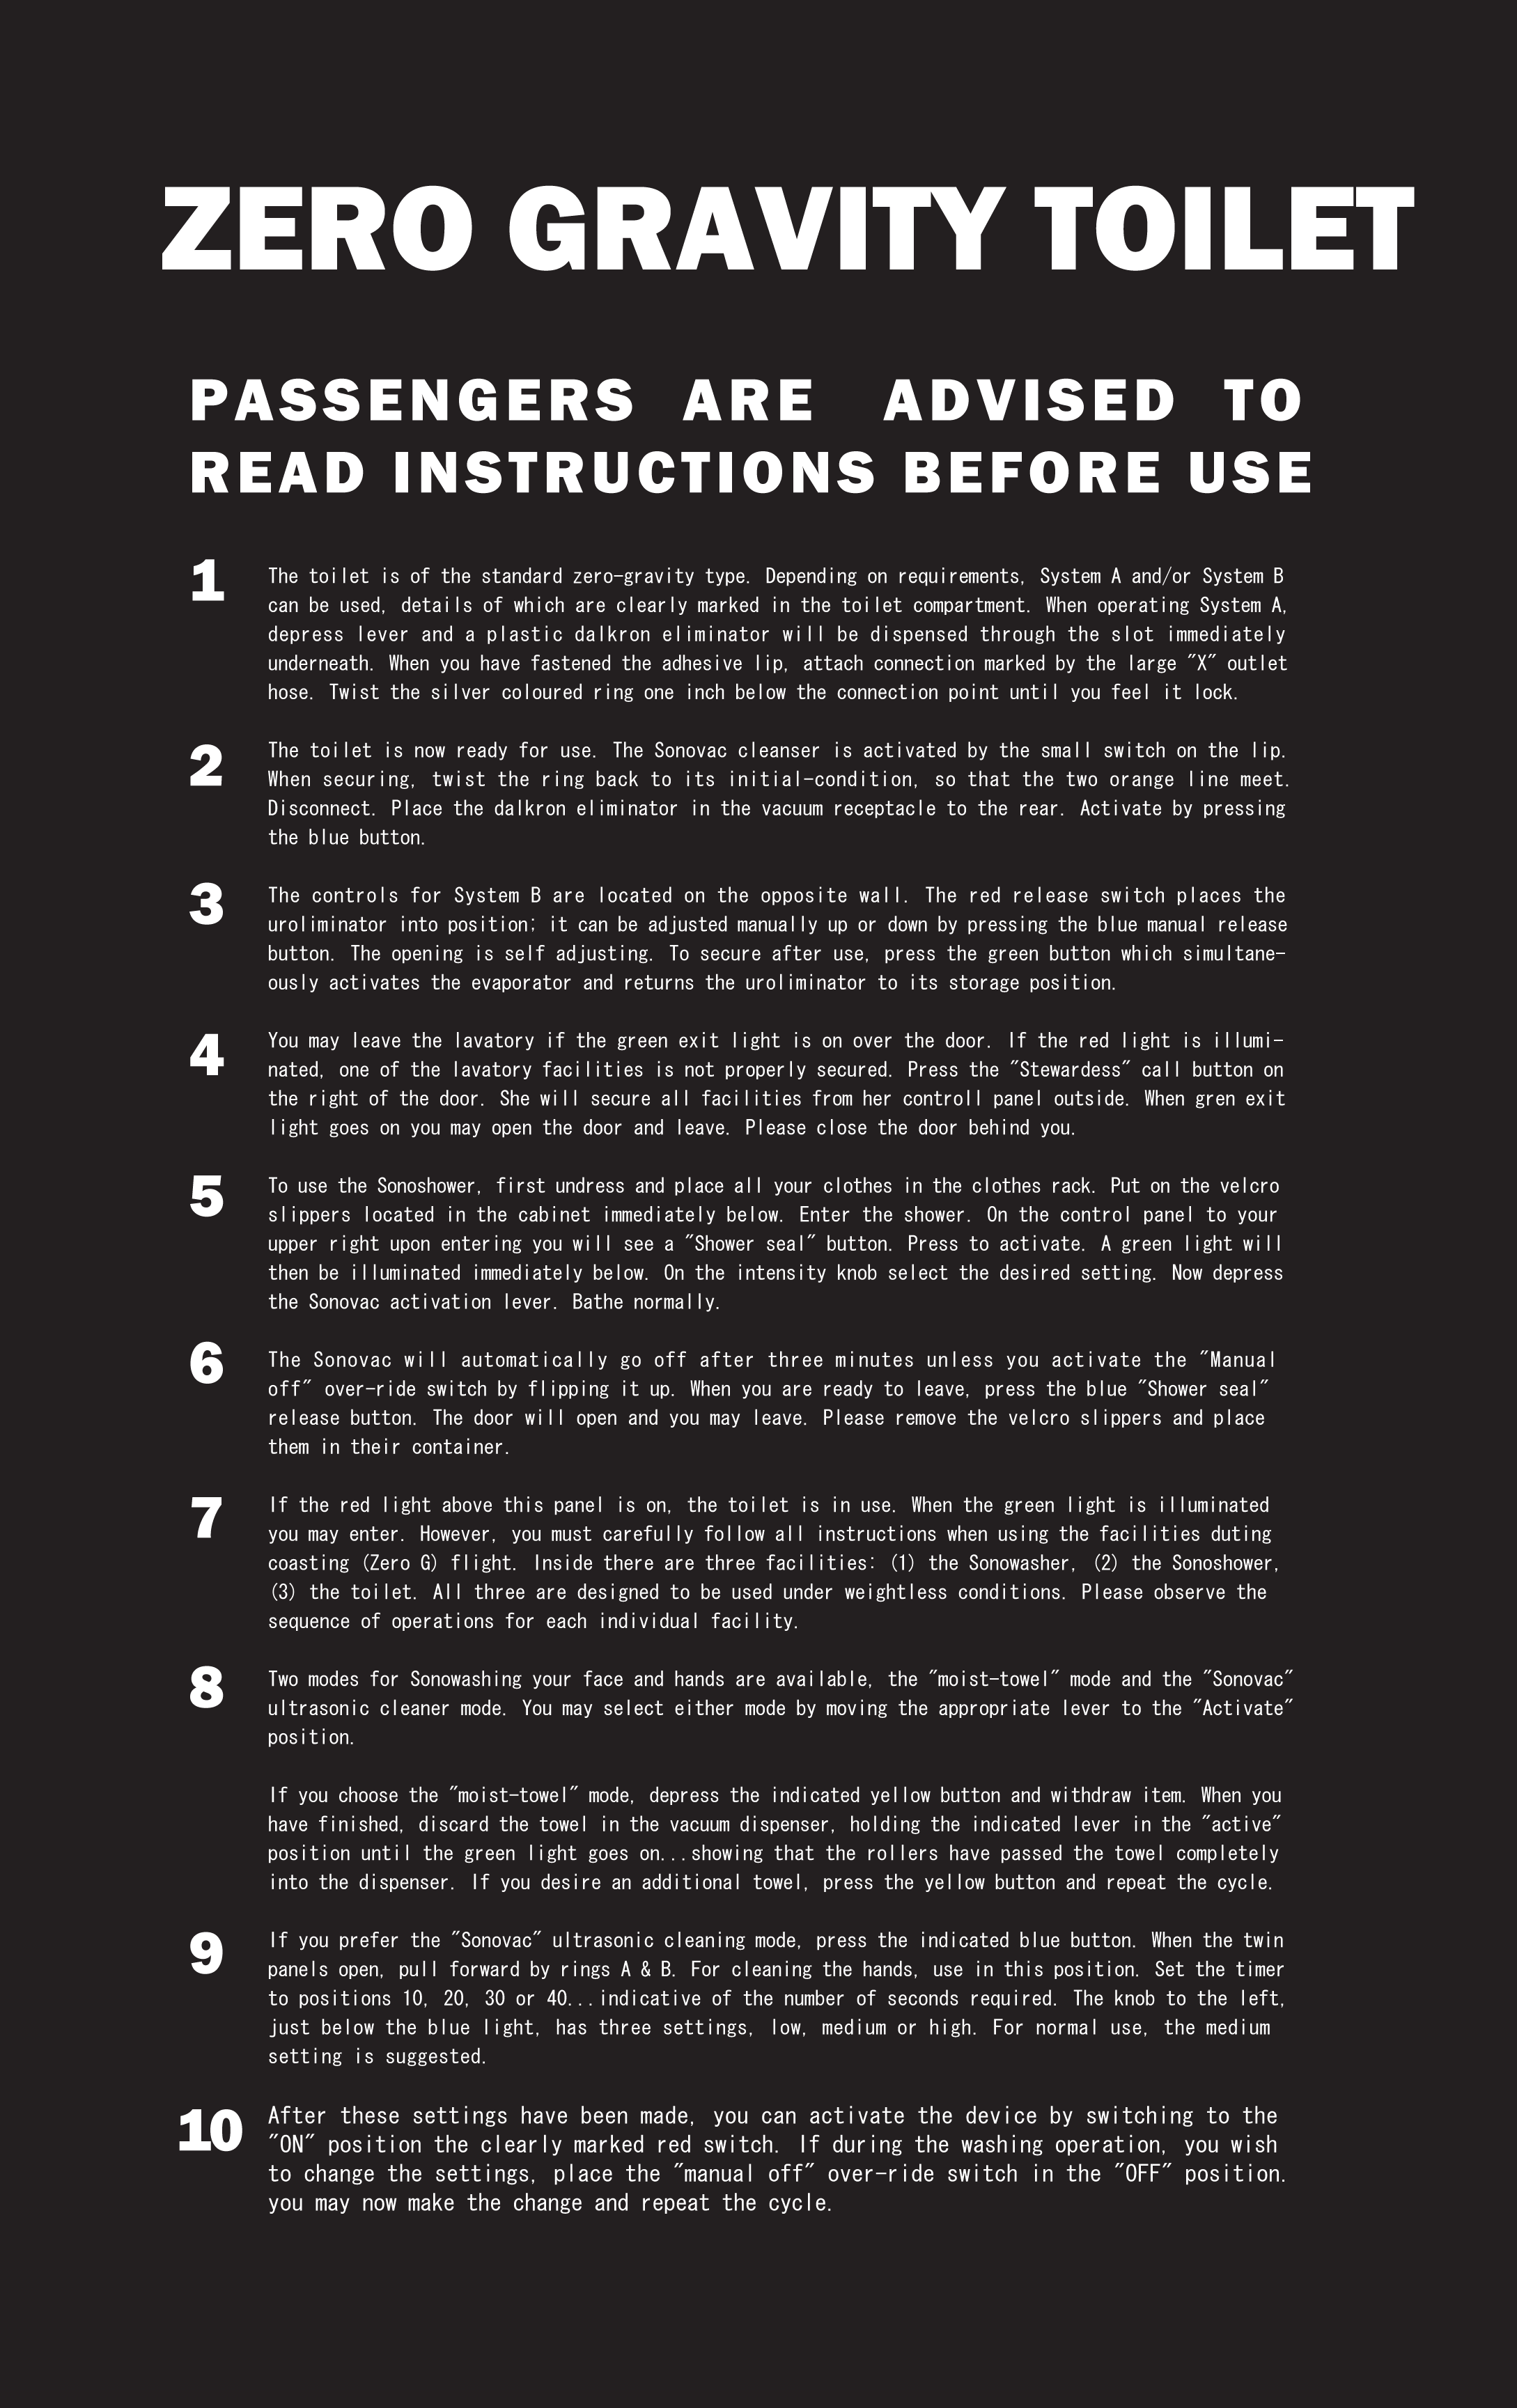
\includegraphics[scale=0.08]{img/002.png}
		\caption{Lista di istruzioni della toilette}
		\label{fig: 002}
	\end{center}
\end{figure}

\noindent\rule{\textwidth}{1pt}
\begin{center}
	\textbf{Toilette di Floyd}
\end{center}

Tendenza del progettista a complicare affari semplici e a pretendere che basti descrivere una procedura per renderla ovvia a qualsiasi utente.

\noindent\rule{\textwidth}{1pt}

\section{Sei concetti centrali}
\paragraph{Definizione classica di interazione (ISO 9241)} \label{par: ISO 9241}
\textbf{Un sistema interattivo} è una combinazione di componenti hardware e software che ricevono input da un utente umano e gli forniscono un output allo scopo di supportare l'effettuazione di un compito.

\begin{figure}[h!]
	\begin{center}
		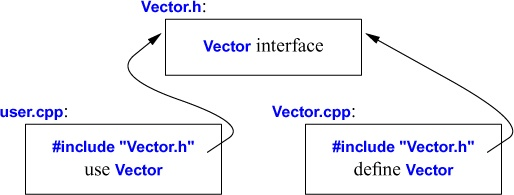
\includegraphics[scale=0.5]{img/003.jpg}
		\caption{Mappa sullo scopo e sul metodo di completamento di un'azione}
		\label{fig: 003}
	\end{center}
\end{figure}

\textbf{Un'interfaccia} è l'insieme dei componenti di un sistema interattivo (software o hardware) che forniscono all'utente informazioni e comandi per permettergli di effettuare specifici compiti attraverso il sistema. \label{par: sistema interattivo}

In comune hanno il concetto di "effettuazione di un compito", da ciò si capisce che il sistema interattivo permette all'utente di conseguire un'obiettivo (compito).

\subsection{Visibilità}
Permette all’utente di individuare facilmente qual è la funzione dell’oggetto, e quindi riconoscere se è adatto allo scopo prefissato. È il risultato dell’applicazione di tutti gli altri principi elencati.

\subsection{Modello concettuale}
É il modello che l’utente ha dell’oggetto in questione; il modello può essere superficiale e riferirsi alla sola conoscenza di relazione tra input e output, ma può anche essere più approfondito, arrivando a conoscere anche tutti i passaggi intermedi a livello macchina. Più il modello concettuale è fedele al funzionamento reale, maggiore è la probabilità di successo nell’interazione tra utente e macchina.

\subsection{Affordance (invito all’uso)} 
Vedere pagina \pageref{par: affordance}.

Gibson: è la risorsa o supporto che l'ambiente offre all'utente

Norman: è una qualsiasi proprietà o qualità di un oggetto che definisce i suoi possibili utilizzi o rende chiaro come possa o debba essere usato.

Una affordance è qualsiasi proprietà di un oggetto che invita una persona competente all'azione mediata da tale oggetto.

\subsection{Significanti}
Tutto ciò che aggiunge ulteriori indicazioni sull’esecuzione dell’azione, come direzione di movimento, senso di rotazione, ecc.

\subsection{Feedback (reazione)}
É l’insieme di risposte che il sistema comunica all’utente, in base alle azioni effettuate fino a quel momento.

\subsection{Mapping} 
Vedere pagina \pageref{par: mapping}.
	
É il rapporto fra i comandi, il loro azionamento ed i risultati che ne derivano nel mondo esterno; permette all’utente di creare un collegamento diretto fra i comandi di controllo e le parti dell’oggetto di cui modificano rispettivamente lo stato.



\section{Affordance} \label{par: affordance}
\noindent\rule{\textwidth}{1pt}
\begin{center}
	\textbf{Affordance (invito all’uso)}
\end{center}
Gibson: è la risorsa o supporto che l'ambiente offre all'utente

Norman: è una qualsiasi proprietà o qualità di un oggetto che definisce i suoi possibili utilizzi o rende chiaro come possa o debba essere usato.

Una affordance è qualsiasi proprietà di un oggetto che invita una persona competente all'azione mediata da tale oggetto.

\noindent\rule{\textwidth}{1pt}

Ci sono vari tipi di affordance:
\begin{itemize}
	\item \textbf{Cognitive}: aiuta gli utenti attraverso le loro capacità cognitive (pensare, decidere, imparare, ricordare e conoscere)
	\item \textbf{Fisiche}: aiuta l'utente attraverso le sue azioni fisiche (cliccare, toccare, puntabile, gesticolare, muovere)
	\item \textbf{Sensoriali}: aiuta l'utente attraverso le sue azioni sensoriali (vedere, sentire e percepire
	\item \textbf{Funzionali}: aiuta l'utente a realizzare il suo compito e a comprendere come usare lo strumento
	\item \textbf{Emotiva}: aiuta l'utente ad esperire certe emozioni (il caso più intuitivo è quello delle emoticon e delle sue evoluzioni) 
	\item \textbf{Sociale}: aiuta l'utente ad esperire certe funzioni sociali
\end{itemize}

Le affordance non sono esclusive, posso copartecipare all'intuizione, il problema è quando sono in contraddizione. Nel caso la progettazione non sia intuitiva gli utenti possono aggiungerle (ad esempio inserendo un cartello).

\section{Mapping} \label{par: mapping}
\noindent\rule{\textwidth}{1pt}
\begin{center}
	\textbf{Mapping}
\end{center}	
É il rapporto fra i comandi, il loro azionamento ed i risultati che ne derivano nel mondo esterno; permette all’utente di creare un collegamento diretto fra i comandi di controllo e le parti dell’oggetto di cui modificano rispettivamente lo stato.

\noindent\rule{\textwidth}{1pt}
\begin{figure}[h!]
	\begin{center}
		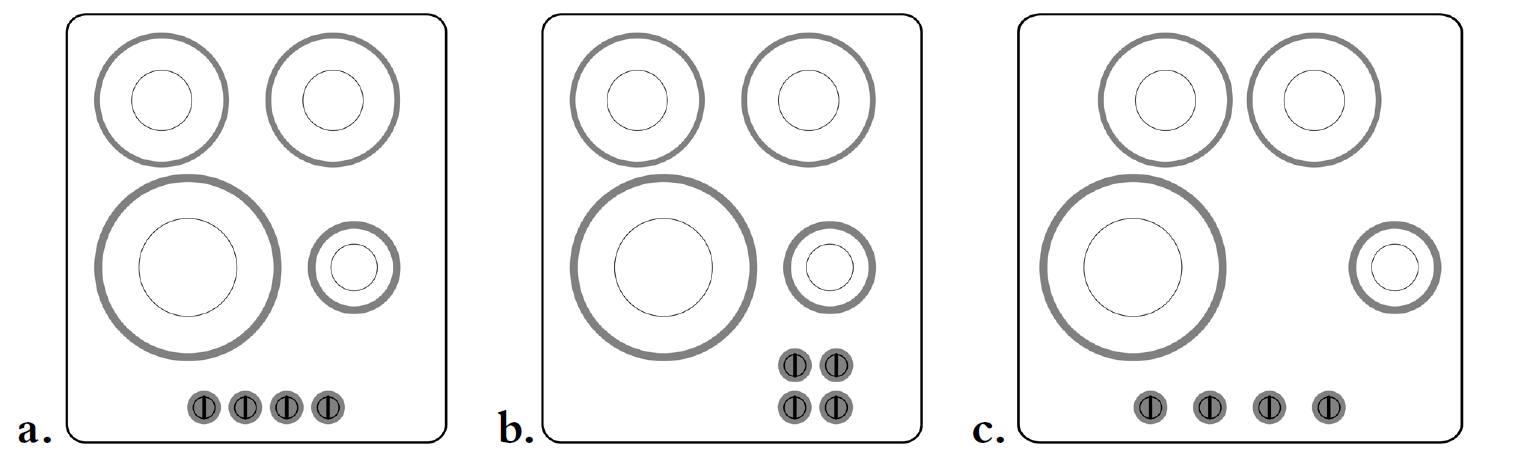
\includegraphics[scale=0.2]{img/006.png}
		\caption{Esempi di mapping topologici mancati e riusciti}
		\label{fig: 006}
	\end{center}
\end{figure}
Come possiamo vedere nell'immagine \ref{fig: 006} il mapping topologico è buono ma quello funzionale, in certi casi, può essere migliorato: cosa ha a che fare la rotazione con l'intensità della fiamma e quindi il calore?

\begin{figure}[h!]
	\begin{center}
		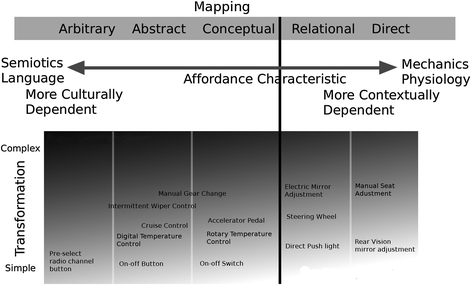
\includegraphics[scale=0.6]{img/007.png}
		\caption{Grafico mapping-affordance}
		\label{fig: 007}
	\end{center}
\end{figure}
Anche per il mapping possiamo averne di semplici e complessi. Dall'immagine \ref{fig: 007} possiamo vedere i tipi di mapping individuati da McLuhan:
\begin{itemize}
	\item \textbf{Arbitrario}: una relazione del tutto immaginata dal progettista e che l'utente adotta solo per prove ed errori e poi impara a memoria, senza riferimenti culturali o indicazioni fisiche
	\item \textbf{Convenzionale}: la relazione tra controllo ed effetto è stabile, quasi ovvia, ma legata a delle convenzioni. Ad esempio solo una convenzione ci permette di capire che la seconda marcia, che in molte automobili si trova nella fila inferiore e comunque sotto la prima marcia, in altre invece sopra, è quella che riduce la coppia alla ruota a parità di coppia del motore
	\item \textbf{Naturale}: la relazione è meno immediata che nel caso diretto (ma i concetti sono molto simili)
	\item \textbf{Diretto}: c'è una relazione fisica, visibile, spesso legata alla posizione, tra controllo (che afforda una azione) e l'effettore controllato che produce un effetto nel mondo
\end{itemize}

Ricordiamo che non si può avere mapping senza affordance ma si può avere affordance senza mapping.

Un'affordance non è solo qualcosa che suggerisce una azione su di essa ma anche qualcosa che suggerisce un possibile effetto sul mondo. è proprio il mappinga, che è una caratteristica dell'affordance, che si occupa di rendere questo collegamento o relazione più o meno semplice da capire.

\subsection{La legge di Fitt}
\noindent\rule{\textwidth}{1pt}
\begin{center}
	\textbf{Legge di Fitts}
	
	$MT = a + b\log_{2}(\dfrac{D}{W} + 1)$ \\dove MT è il tempo di movimento, D è la distanza dall'obiettivo e W è la grandezza dell'obiettivo
\end{center}
\begin{figure}[h!]
	\begin{center}
		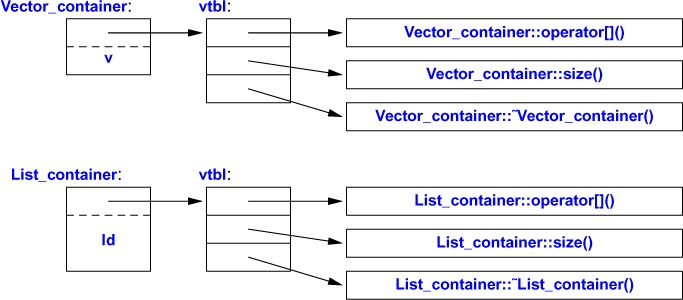
\includegraphics[scale=0.6]{img/004.jpg}
		\caption{Legge di Fitt}
		\label{fig: 004}
	\end{center}
\end{figure}
\noindent\rule{\textwidth}{1pt}

Nella progettazione si può pensare di rendere più efficienti per la legge di Fitt le funzioni più frequenti e rendere meno efficienti quelli per i quali serve una forma di sicurezza.

\section{Scheumorfismo}
Uno scheumorfismo è un ornamento fisico o grafico apposto su un oggetto allo scopo di richiamare le caratteristiche estetiche di un altro. Un esempio è la calcolatrice digitale che cerca di replicare gli schemi che ritroviamo su quelle fisiche, oppure all'applicazione di un e-reader che simula il girare fisicamente la pagina.

\begin{figure}[h!]
	\begin{center}
		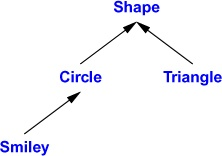
\includegraphics[scale=0.6]{img/005.jpg}
		\caption{Esempio di scheumorfismo}
		\label{fig: 005}
	\end{center}	
\end{figure}

Perchè oggi non viene più usato così pervasivamente? Perchè spesos questo approccio può essere estremamente utile per permettere all'utente un'interazione veloce ma porta con sè eventuali costi di performance. Oggi è stato sostituito da un approccio più flat. 

Lo scheumorfismo può anche portare il problema di essere vincolati troppo dall'oggetto fisico.

\section{Vincoli e workaround}
Un vincolo può essere:
\begin{itemize}
	\item \textbf{passivo/concettuale}: ad esempio concepisco un form con tre campi e non quattro, per vincolare l'inserimento di soli tre tipi di dato; non prevedo un campo "note", non prevedo un canale di ritorno (feedback) tra consumatore e azienda
	\item \textbf{attivo/funzionale}: ad esempio concepisco dei controlli per cui l'utente non può proseguire se non compila tutti i campi, o non li compila "correttamente" sulla base di regex come ad esempio per l'indirizzo mail o il codice fiscale)
\end{itemize}

I vincoli vanno sempre bene? No, se l'utente si sentisse troppo vincolato potrebbe iniziare a creare dei workaround. Questi vengono chiamati "desire path".

\noindent\rule{\textwidth}{1pt}
\begin{center}
	\textbf{Desire Path}
\end{center}

Qualsiasi azione relativa all'esecuzione di un processo o di un compito (supportati dal sistema informatico) che non è prevista o descritta nei manuali di uso del sistema informatico e/o nei manuali che descrivono tale processo o procedura e che può bypassare l'uso del sistema o piegarlo ai propri fini.

"Percorso del desiderio", sono quei percorsi di interazione che descrivono il percorso ideale da parte dell'utente.

\noindent\rule{\textwidth}{1pt}

\section{Progettare per affordance} \label{par: complessità}
\begin{itemize}
	\item Seguire le maggiori convenzioni già stabilite per immagini e azioni ed adottare un mapping naturale il più spesso possibile
	\item Se appropriato, usare parole in aggiunta alle icone e alle grafiche
	\item usare metafore riconoscibili (ad esempio il cestino dei rifiuti per indicare il cancellare un file)
	\item Essere consistenti e coerenti nell'uso dei modelli concettuali usati durante la fase di design (banalmente l'usare sempre la stessa dicitura per il tasto di conferma)
\end{itemize}

\begin{figure}[h!]
	\begin{center}
		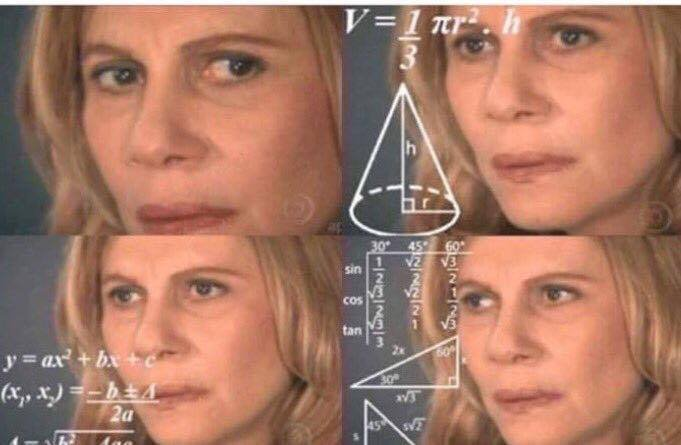
\includegraphics[scale=0.6]{img/008.jpg}
		\caption{Mappa complessità funzionale e strutturale}
		\label{fig: 008}
		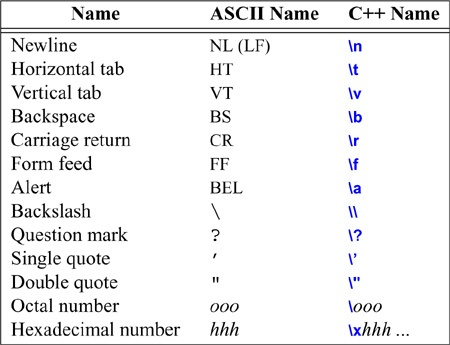
\includegraphics[scale=0.6]{img/009.jpg}
		\caption{Mappa complessità funzionale e d'uso}
		\label{fig: 009}
	\end{center}
\end{figure}
\begin{itemize}
	\item \textbf{Complessità funzionale}: indica quante funzioni possono essere svolte tramite l'interfaccia in analisi (un cacciavite a punta singola ha una bassa complessità funzionale, un coltellino svizzero ha un'alta complessità funzionale in quanto in base a come viene usato può svolgere numerose funzioni in virtù delle sue componenti)
	\item \textbf{Complessità strutturale}: indica, genericamente, quanto sia complessa la struttura di uno strumento (un cucchiaio ha una complessità strutturale bassa, uno smartphone una complessità strutturale alta)
	\item \textbf{Complessità d'uso}: indica quando sia semplice utilizzare l'interfaccia, ha un forte elemento basato anche sulle capacità personali (una maniglia ha complessità d'uso bassa, una macchina con cambio manuale ha complessità d'uso alta)
\end{itemize}

Il nostro obiettivo è raggiungere alta complessità funzionale con bassa complessità d'uso. Ci sono degli accorgimenti che ci permettono di diminuire la complessità d'uso, ad esempio una progettazione oculata.

\subsection{Perchè è necessario semplificare l'uso?}
Prima di tutto la pervasività della tecnologia al giorno d'oggi ci richiede ciò, se fosse complicata da usare ci sarebbero più difficoltà nella sua implementazione nella vita di tutti i giorni.

L'accessibilità è un altro capo saldo, renderla usabile e accessibile a tutti, non solo in termine di rimozione di barriere architettoniche ma in generale come possibilità d'accesso, non bloccata da limiti fisici o di disponibilità.

C'è anche la necessità di comprendere ruoli e possibilità della tecnologia per migliorare la qualità della vita.

Le interfacce non sono solo il mezzo interattivo con i sistemi ma sono anche un filtro della complessità d'uso, una buona interfaccia semplifica l'utilizzo e da qua l'integrazione. La capacità di creare un sistema con una minore complessità d'uso ci permette di essere competitivi.

\chapter{Valutazione di usabilità}
\section{In cosa consiste il progetto?}
\textbf{Chi è coinvolto}? Noi e utenti reali

\textbf{Che tipi di analisi ci sono?}
\begin{itemize}
	\item Confronto longitudinale: nel tempo
	\item Confronto trasversale: tra due opzioni
\end{itemize}
\textbf{Quali sono gli step?}
\begin{figure}[h!]
	\begin{center}
		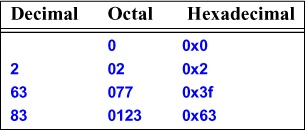
\includegraphics[scale=0.55]{img/010.jpg}
		\caption{Gli step per i due confronti}
		\label{fig: 010}
	\end{center}
\end{figure}
\textbf{Valutazione euristica}: 3 utenti esperti di dominio + 3 utenti esperti di usabilità (cioè noi). Per utenti esperti di dominio si intendono utenti che usano abitualmente il tipo di interfaccia in analisi.

\textbf{User test}: i 12 utenti tra i 24 che saranno coinvolti negli user test devono essere più rappresentativi possibili della popolazione utilizzatrice.

Durante lo user test bisogna registrare l'interazione (c'è un modulo apposito per la privacy).

\section{Valutazione euristica (qualitativa)} \label{par: euristica}
Si coinvolgono utenti (esperti del task) e/o esperti di usabilità (inclusi noi stessi).

Per valutare sistemi interattivi, a qualsiasi livello di prototipazione e maturità alla luce dei principi di buona progettazione.

Qualitativa non si intende in modo vago ma dove non viene prodotto un numero come output ma invece farsi un'idea sufficientemente completa dei possibili problemi di usabilità.

\begin{figure}[h!]
	\begin{center}
		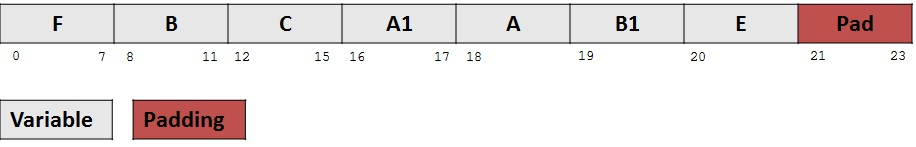
\includegraphics[scale=0.6]{img/012.jpg}
		\caption{Mappa expertise}
		\label{fig: 012}
	\end{center}
\end{figure}
Per tutti gli utenti bisogna includere all'interno della relazione una mappa che interpoli expertise di dominio e sulla usabilità e posizioni gli utenti coinvolti su di questa (una mappa come nella figura \ref{fig: 012}.

L'expertise sull'usabilità è quella riguardante cosa si conosce dei buoni principi di progettazione, quella sul dominio è l'expertise nell'applicazione specifica.

La valutazione euristica è la valutazione (di usabilità) svolta alla luce di un determinato insieme di euristiche (ben definite, possibilmente ben note, prese a riferimento) per identificare soluzioni di design che o si conformano o violano una o più euristiche di tale insieme.

\subsection{Quali indicazioni per il design dell'interfaccia utente?}
\begin{figure}[h!]
	\begin{center}
		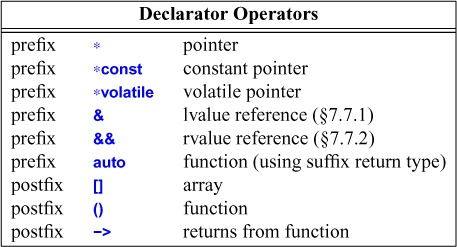
\includegraphics[scale=0.6]{img/013.jpg}
		\caption{Tipi di principi e linee guida}
		\label{fig: 013}
	\end{center}
\end{figure}

Si chiamano anche principi euristici o semplicemente "euristiche". Una euristica è quindi un insieme di concetti, riferimenti e, soprattutto, strategie che si sono rilevate particolarmente adatte a risolvere un determinato problema, nel nostro caso la progettazione di sistemi interattivi usabili.
\subsubsection{Principi}
Indicazioni generali per la progettazione di interfacce utente usabili, basate su evidenza scientifica o sul generale consenso. Derivano dalla conoscenza degli aspetti psicologici, computazionali e sociali e sono indipendenti dalla tecnologia. Sono espressi spesso in forma molto generale.

\subsubsection{Standard}
Insieme di regole da applicare nel progetto di una classe di sistemi. possono essere vincolanti. Sono di norma emesse da un Ente di standardizzazione (e.g. ISO). La conformità allo standard deve essere valutabile in modo preciso. (Vedere \pageref{par: ISO 9241}

\subsubsection{Linee guida e design patterns}
Insieme di raccomandazioni per il progetto dell'interfaccia utente per una particolare classe di sistemi, espresse in modo generale ma meno astratte dei principi, con esempi e motivazioni. Non sono mai vincolanti, sta al progettista decidere sulla opportunità per applicarle caso per caso.

Il concetto di "design pattern" nasce in architettura. Si tratta di riutilizzare buone pratiche (appunto raccomandazioni) per non dovere reinventare tutto da capo. Per i programmatori i più famosi sono \href{https://refactoring.guru/design-patterns}{i design pattern pensati dalla GoF}. Diffondono standard testati e facilitano la formazione di un linguaggio comune.

\subsubsection{Regole di progetto}
Insieme di regole o specifiche da applicare nel progetto di un particolare sistema. Sono vincolanti all'interno del progetto, ad esempio perchè dettate da precisi requisiti del cliente/committente o per motivi di budget e vincoli progettuali.


Si usano i principi e non le linee guida perchè non vogliamo essere vincoli eccessivi. 
\subsection{Livelli di autorevolezza dei principi}
Ci sono diversi livelli di autorevolezza dei principi (o forza dell'evidenza):
\begin{enumerate}
	\item Completamente supportati da risultati di ricerca e dati empirici
	\item Basati su pratica generalmente accettata (in modo documentato)
	\item Non ben documentate, ma supportate dall'opinione di professionisti esperti
	\item Opinione individuale
\end{enumerate}

Solo i primi due gradi sono recepiti. I principi di Nielsen sono tra B e C, alcune soluzioni specifiche (ispirate a quei principi) anche di livello A.

\chapter{Lessico}
\paragraph{Ergonomia}
Disciplina scientifica che si occupa dei problemi relativi al lavoro umano in rapporto alla progettazione delle macchine e agli ambienti di lavoro, al fine di individuare le soluzioni più idonee alle esigenze psicofisiche dei lavoratori e al contempo a quelle della produzione.

\paragraph{Sistema socio tecnico}
Pagina \pageref{par: sistema sociotecnico}.

\begin{itemize}
	\item è un sistema, "un insieme di elementi interrelati ed eventualmente mutuamente dipendenti che, agli occhi di un osservatore esterno, appaiono come un'entità unitaria ma collettiva, con caratteristiche e comportamento proprio, solitamente autonomo ed intenzionale (cioè volto ad un obiettivo)";
	\item Un sistema in cui la componente umana  (sociale) e quella tecnica (tecnologica) sono inestricabilmente legate tra loro e la loro interazione porta a fenomeni emergenti impredicibili. Attenzione che tecnica è un termine generico proprio per intendere tutti gli strumenti, che siano fisici o dell'ingegno. In più si parla di interdipendenza perchè lo strumento è fermo senza qualcuno che lo usa, l'umano è fermo se non ha uno strumento per agire;
	\item è un concetto di invarianza di scala, ovvero il concetto non cambia in base alla grandezza dell'ambiente sociale
\end{itemize}

\paragraph{Affordance}
Pagina \pageref{par: affordance}.
Gibson: è la risorsa o supporto che l'ambiente offre all'utente

Norman: è una qualsiasi proprietà o qualità di un oggetto che definisce i suoi possibili utilizzi o rende chiaro come possa o debba essere usato.

Una affordance è qualsiasi proprietà di un oggetto che invita una persona competente all'azione mediata da tale oggetto.

\paragraph{Mapping}
Pagina \pageref{par: mapping}.

É il rapporto fra i comandi, il loro azionamento ed i risultati che ne derivano nel mondo esterno; permette all’utente di creare un collegamento diretto fra i comandi di controllo e le parti dell’oggetto di cui modificano rispettivamente lo stato.
\paragraph{Porte di Norman}
Pagina \pageref{par: porta di norman}.

Una porta di Norman è una porta il cui design suggerisce un'azione contraria a quella da fare o che richiede un segnale per spiegare come usarla.

\paragraph{Toilette di Floyd}
Pagina \pageref{par: toilette di Floyd}.

Una toilette di floyd è un qualcosa di progettato in maniera così poco intuitiva per il quale devo fornire una serie di istruzioni.

\paragraph{Sistema interattivo e interfaccia}
Pagina \pageref{par: sistema interattivo}.

Per interfaccia d'uso (o interfaccia utente, user interface) intendiamo l'insieme di “tutti i componenti di un sistema interattivo (software o hardware) che forniscono all'utente informazioni e comandi per permettergli di effettuare specifici compiti attraverso il sistema.

\paragraph{Automation bias/overreliance}
Pagina \pageref{par: automation bias}.

è l'eccessiva fiducia nella risposta del supporto alle decisioni e quindi causa di errori di omissione o di azione quando i sistemi sono imperfetti (e.g. la calcolatrice che deve rispondere correttamente, non può essere altrimenti). è legato ai processi decisionali.

\paragraph{Errori di giustapposizione}
Quando a causa della posizione specifica di un elemento si preme un pulsante differente rispetto a quello desiderato (e.g. due elementi in un menù a tendina che sono molto vicini tra loro)

\paragraph{Complessità strutturale, funzionale e d'uso}
Pagina \pageref{par: complessità}.

\begin{itemize}
	\item \textbf{Complessità funzionale}: indica quante funzioni possono essere svolte tramite l'interfaccia in analisi (un cacciavite a punta singola ha una bassa complessità funzionale, un coltellino svizzero ha un'alta complessità funzionale in quanto in base a come viene usato può svolgere numerose funzioni in virtù delle sue componenti)
	\item \textbf{Complessità strutturale}: indica, genericamente, quanto sia complessa la struttura di uno strumento (un cucchiaio ha una complessità strutturale bassa, uno smartphone una complessità strutturale alta)
	\item \textbf{Complessità d'uso}: indica quando sia semplice utilizzare l'interfaccia, ha un forte elemento basato anche sulle capacità personali (una maniglia ha complessità d'uso bassa, una macchina con cambio manuale ha complessità d'uso alta)
\end{itemize}

\paragraph{Euristica e valutazione euristica}
Pagina \pageref{par: euristica}.

Una euristica è un insieme di concetti, riferimenti e, soprattutto, strategie che si sono rilevate particolarmente adatte a risolvere un determinato problema, nel nostro caso la progettazione di sistemi interattivi usabili.

La valutazione euristica è la valutazione (di usabilità) svolta alla luce di un determinato insieme di euristiche (ben definite, possibilmente ben note, prese a riferimento) per identificare soluzioni di design che o si conformano o violano una o più euristiche di tale insieme.

\paragraph{Segno, simbolo, indice, icona}
\paragraph{Significante, significato, oggetto}
\paragraph{Metacomunicazione}
\paragraph{Deputy del progettista}
L'oggetto creato rappresenta l'artista che lo crea.
\paragraph{Captologia}
\paragraph{Soggettivismo - oggettivismo}
\section{"Metodologia"}
\begin{figure}[h!]
	\begin{center}
		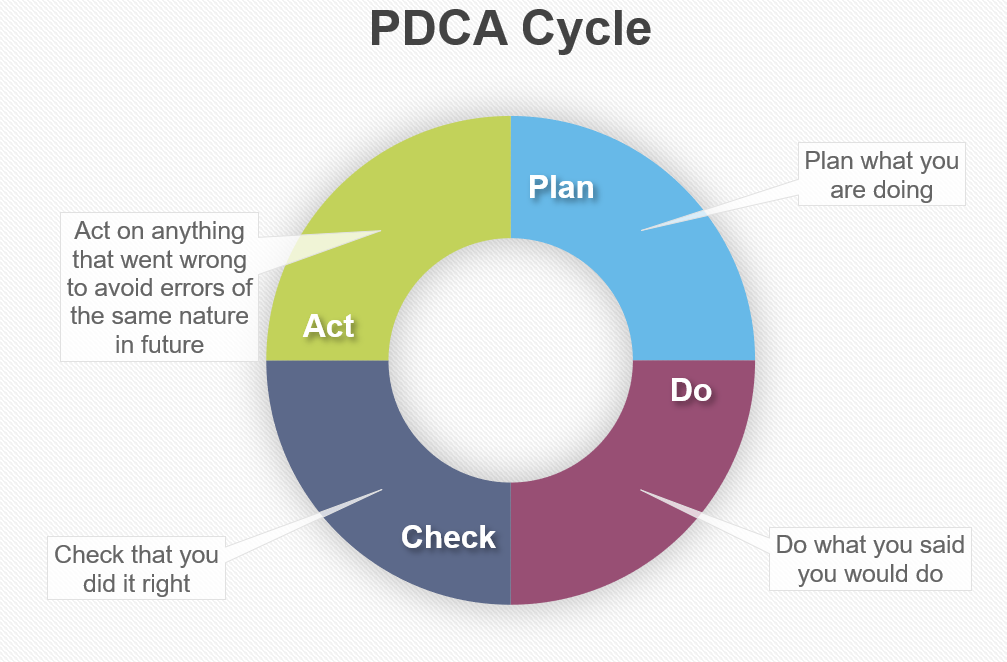
\includegraphics[scale=0.6]{img/011.png}
		\caption{PDCA cycle}
		\label{fig: 011}
	\end{center}
\end{figure}
\begin{itemize}
	\item Affina sensibilità per il brutto e il cattivo
	\item Progetta in equilibrio tra familiarità e originalità
	\item Sappi che parli all'utente anche di te stesso
	\item Non guardarti l'ombelico ma coinvolgi gli utenti
	\item Trova i problemi, prioritizzali e risolvili
	\item Valuta usabilità in termini di efficienza, efficacia e soddisfazione
	\item Migliora il tuo artefatto
	\item Torna agli utenti
\end{itemize}

\end{document}
